\documentclass[journal, 10pt]{IEEEtran}
% *** CITATION PACKAGES ***
\usepackage{textcomp}
\usepackage{cite}

\usepackage[none]{hyphenat}

\usepackage{filecontents}
\usepackage{amssymb}

% *** GRAPHICS RELATED PACKAGES ***
%
\ifCLASSINFOpdf
  \usepackage[pdftex]{graphicx}
\else
   \usepackage[dvips]{graphicx}
    % \DeclareGraphicsExtensions{.eps}
\fi
\usepackage{graphicx}

% *** MATH PACKAGES ***
\usepackage[cmex10]{amsmath}
% Also, note that the amsmath package sets \interdisplaylinepenalty to 10000
% thus preventing page breaks from occurring within multiline equations. Use:
%\interdisplaylinepenalty=2500 after loading amsmath to restore such page breaks as IEEEtran.cls normally

% *** ALIGNMENT PACKAGES ***
\usepackage{array}
\usepackage{booktabs}
\usepackage{multirow}

% *** SUBFIGURE PACKAGES ***
\ifCLASSOPTIONcompsoc
  \usepackage[caption=false,font=normalsize,labelfont=sf,textfont=sf]{subfig}
\else
  \usepackage[caption=false,font=footnotesize]{subfig}
\fi
 %subfig.sty
% *** FLOAT PACKAGES ***
\usepackage{float}
\usepackage{stfloats}
\usepackage{hyperref}

\renewcommand{\citedash}{--}

\begin{document}
\title{Virtual Simulation for Testing Robotic Control Architectures for Autonomous Rendezvous Docking }

\author{John Karasinski, Christopher Lorenzen, and Melanie Stich\\Department of Mechanical \& Aerospace Engineering\\University of California, Davis\\Davis, CA, USA }

\maketitle

\begin{abstract}
With small failures leading to the loss of an entire spacecraft, innovations in inspection methods are required.  The viability of a small inspection satellite with a deliberative or a reactive robotic architecture is discussed and methods for testing the robustness of these systems are developed.  Some past docking and machine vision examples in the field are presented as well as their applicable contributions.  A navigation system based primarily on machine vision position determination is used to compare the success of two different control system architectures.  Each of the two architectures are applied to the same environment, and varying initial states and errors are used to test their ability to adapt to different applications or situations.  The fuel burned and time to target are used to quantify the relative performance of the two architectures.  The proposed test environment and simulation methods are introduced to serve as a means for acquiring data to develop empirical cause and effect relationships between the different control design parameters.
\end{abstract}

% Note that keywords are not normally used for peerreview papers.
\begin{IEEEkeywords}
robots, satellite, machine vision, docking, navigation, deliberate, adaptive
\end{IEEEkeywords}


\section{Introduction}

\subsection{Background}
In recent years the small satellite platform has increased in popularity. With the ability to launch multiple small satellites as a secondary payload and the relatively low development cost involved, they are one of the most viable testbeds for new technologies.  One great example of this is the class of satellites that adhere to the CubeSat standard~\cite{CubeSat}.   CubeSat initiatives have made many projects possible due to the minimal costs required.  Although a small size limits their capabilities, higher fidelity projects usually require a larger volume to contain all desired systems.  There are several projects that use slightly larger free flyers that have produced unique navigation demonstrations such as AERCam Sprint, Mini-AERCam, and SPHERES ~\cite{Aercam, MiniAercam, SPHERES}. An obvious limitation to small satellites is the ability to fit all required architecture within the size restrictions set by the design.  One way to reduce the space required is to choose your subsystems such that some may fill multiple roles.  An example of this is to use a science instrument to collect navigation data.  More specifically, an optical sensor can be used to take stereoscopic visual recordings for inspection purposes, and to determine the position and attitude in relation to a target.  To do this, the image captured must be used in conjunction with a machine vision algorithm in order to estimate navigational parameters.

The decision to use stereoscopic visual sensors to inspect was chosen to increase ease of inspection for a human operator.  Using stereo vision and the full visual light spectrum, a more familiar virtual image is produced.  Operators are able to view the subject as if it was in front of them, allowing for quick and informed decision making.  This, as among other reasons, has been realized by many research teams and can be seen in many projects such as SPHERES VERTIGO and the aforementioned AERCam projects~\cite{Aercam,MiniAercam, Vertigo1}.
\begin{figure}[tb]
\begin{center}
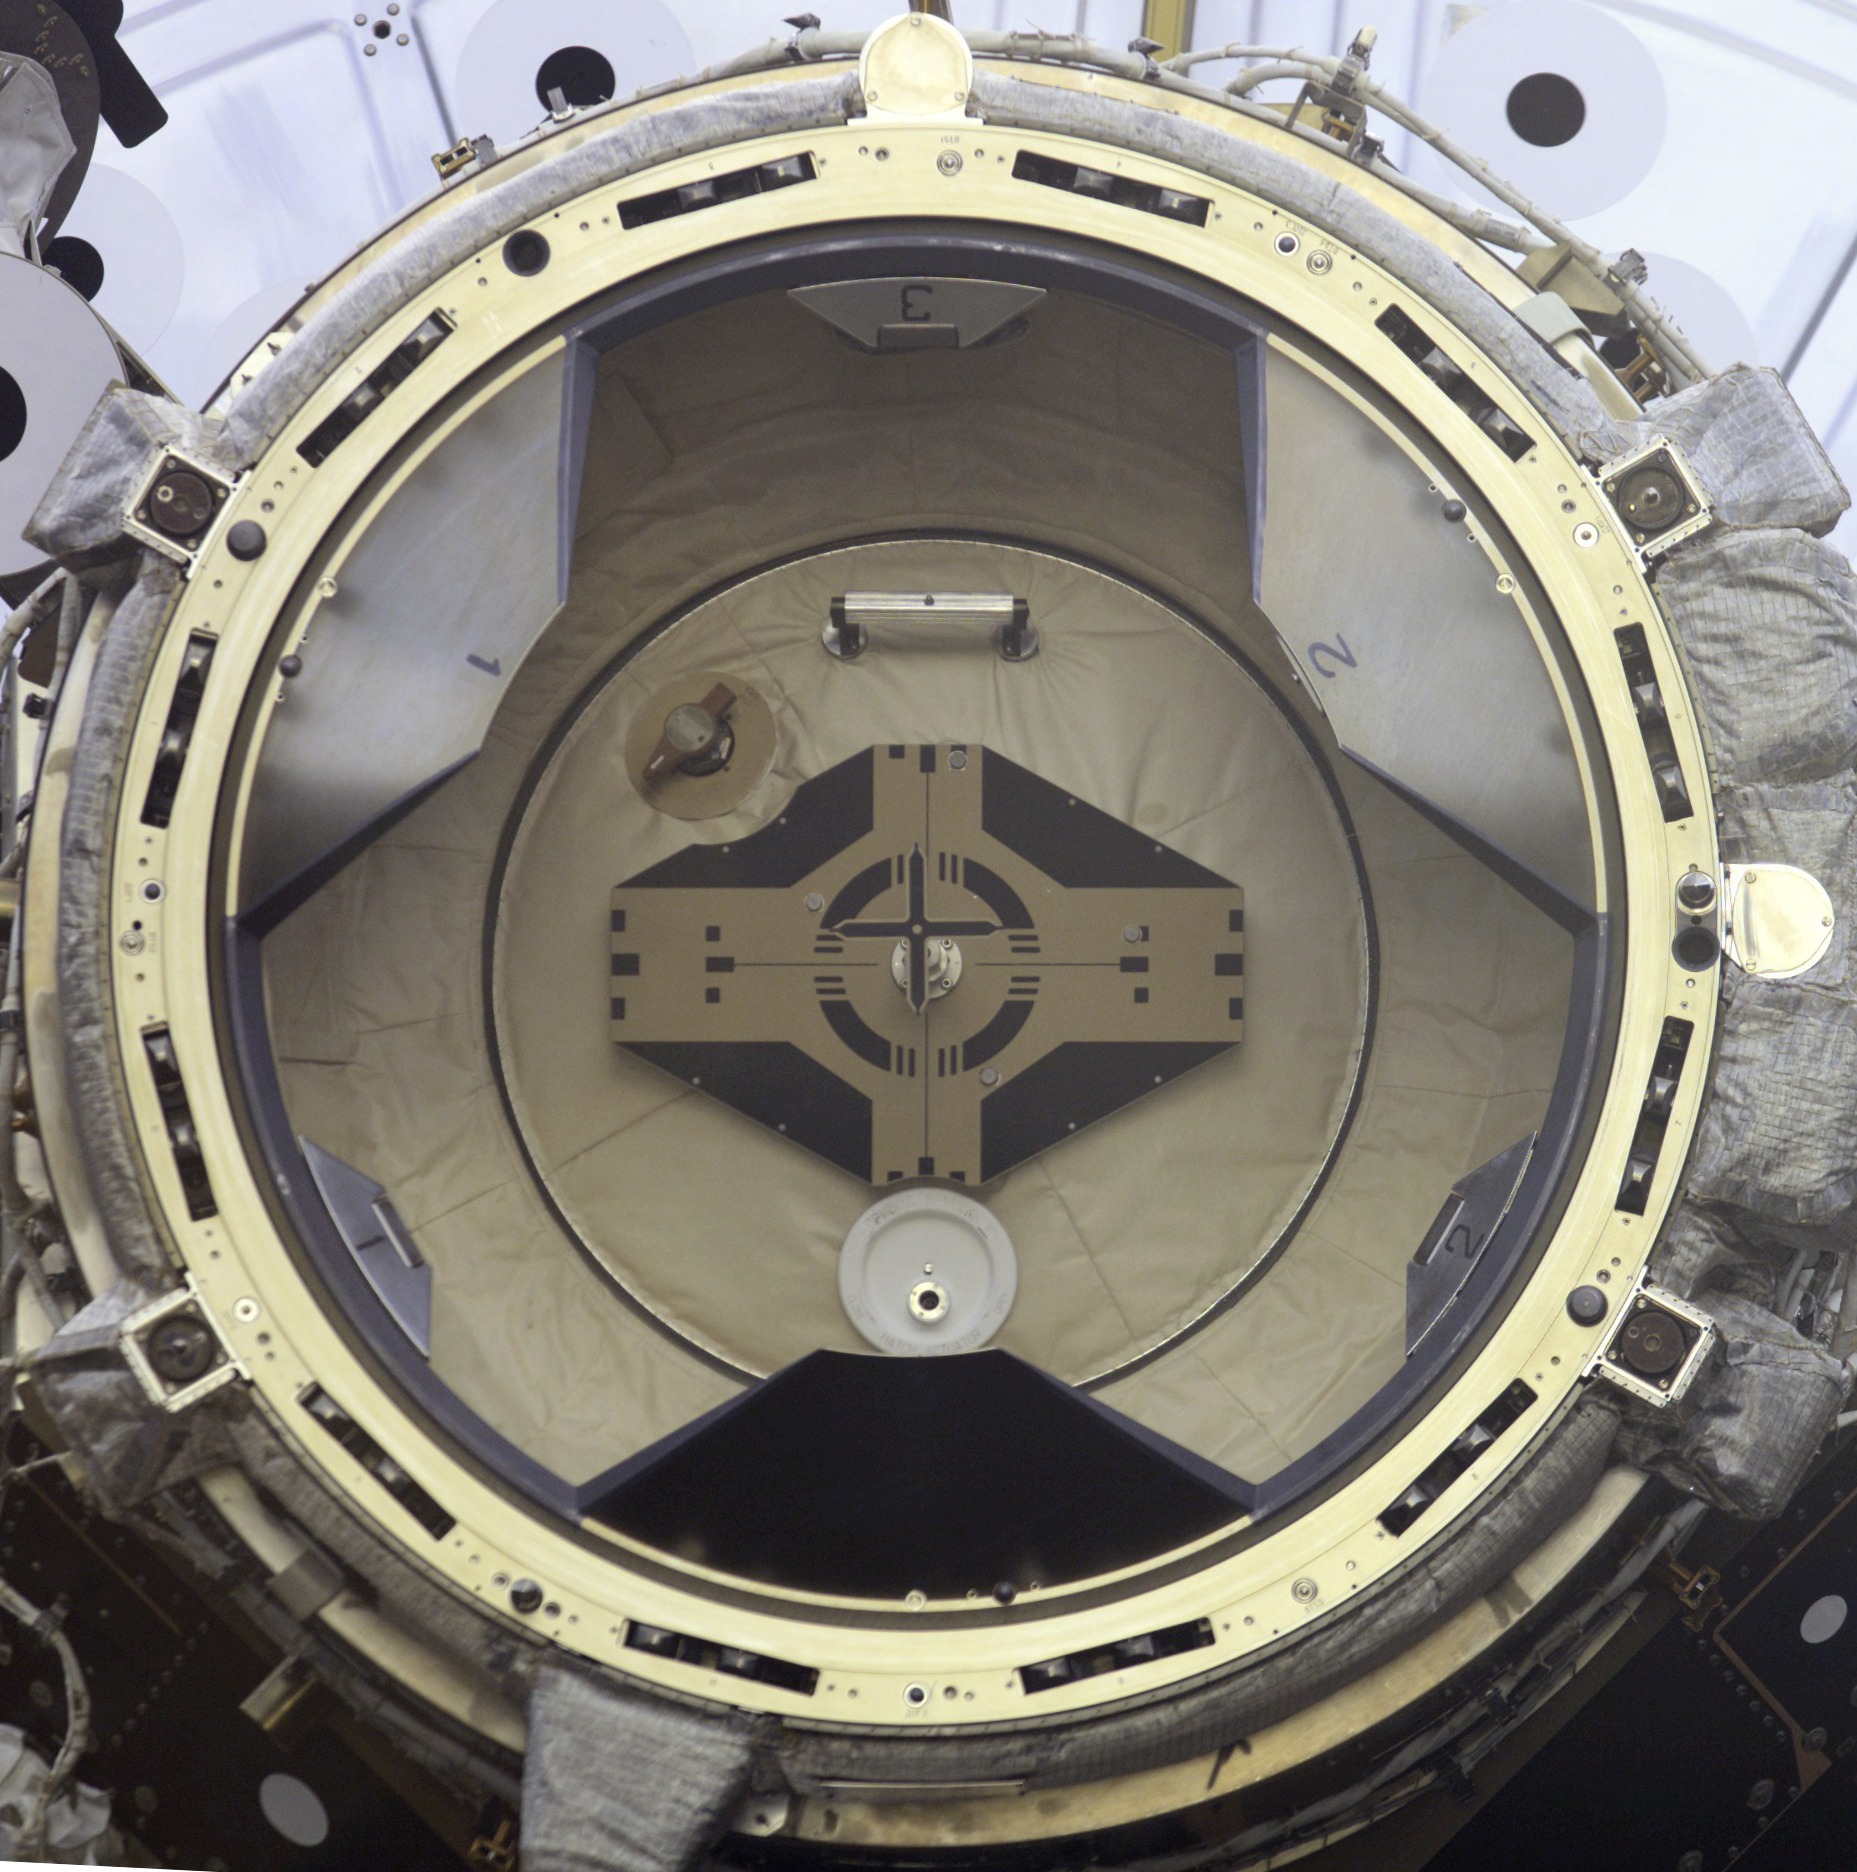
\includegraphics[width=0.37\textwidth]{figures/Docking}
\caption{Visual docking reference with high visibility markers}
\label{VisualDock}
\end{center}
\end{figure}

The ability to dock to the target craft could greatly increase the effective mission operation time, allowing the inspector to refuel, recharge, and download data.  Instead of a small disposable craft that has a single use, it could become a long term asset and an integral part of the target craft's diagnostic routines.  Most current docking procedures utilize a laser range finder for determining distance.  Laser range finders have flight heritage and have moderate accuracy~\cite{Docking}.  Simple fiducial markers can be used to increase the performance of rangefinders, and multiple markers can allow rangefinders to triangulate a relative position.  Markers for visual navigation systems, however, can vary in complexity.  Marker distribution and marker shape can allow a machine vision system to gather a large amount of data with a single image, whereas a laser rangefinder must take multiple measurements.  An example of visual cues for docking can be seen in Figure~\ref{VisualDock}.  The alignment markers clearly display position error.  This system was originally developed for manual docking operations, but it also provides visual information to allow more accurate machine vision position measurements.



\subsection{Motivation}
The advantages presented by the addition of an inspector satellite to a larger craft show the necessity for the development of this technology.  Whether the target craft is inhabited by astronauts or not, it can still increase the probability of completing a mission successfully.

There are two main types of damage that can lead to concern.  The first cause for alarm is physical damage due to collision with orbital debris or micrometeorites.  The second is component failure.  Either of these events can be disastrous to a mission.  The best case scenario is that the craft is not inhabited and the only loss is a multimillion dollar piece of equipment.  With inspection capabilities, damage and failures can be identified in a timely manner.  The possibility of salvaging the mission increases greatly with more information about the problem area and additional time. Additional opportunities would arise if inspection capabilities were to be integrated with other projects like DARPA's Phoenix Satellites~\cite{Phoenix}.  The Phoenix project's goal is to have a cluster of modular ``satlets'' rendezvous and integrate with an inoperative target craft.  An inspector could be sent beforehand, or with the satlets, to increase the success rate of the Phoenix's mission.  If damage or component failure could be accurately identified, then the Phoenix system could dock and efficiently repair or repurpose a damaged satellite.

Using the International Space Station as an example, NASA has shown concern for both damage types that could be observed with a visual inspector.  Numerous studies have been conducted, attempting to quantify the danger involved with debris collision~\cite{Risk}.  As seen in Figure~\ref{ISS_risk}, the impact risk for different parts of the station have already been determined and an inspection satellite could be made to center its efforts in patrolling high risk areas.  There have also been close calls due to component failures.  One such incident requiring emergency extra-vehicular activity was when an ammonia pump developed a leak in May 2013~\cite{Ammonia}.

\begin{figure}[tb]
\begin{center}
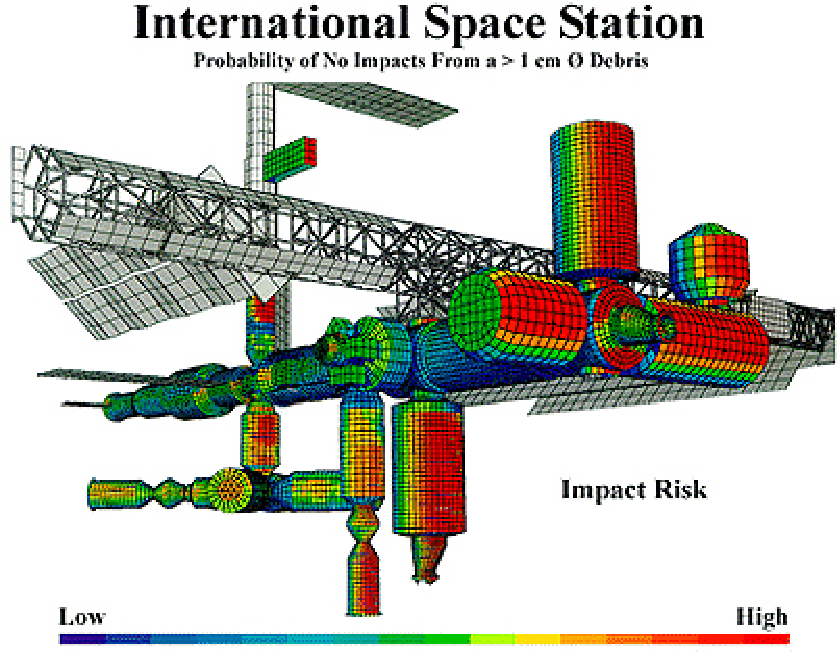
\includegraphics[width=0.4\textwidth]{figures/ISS_impact_risk}
\caption{Debris impact risk by region of the International Space Station}
\label{ISS_risk}
\end{center}
\end{figure}

Beyond the overall need for an inspection resource, there is also a driving factor to attain efficiency.  With increased navigational efficiency, it extends the life of the inspector as well as increasing the amount of data that can be gathered with each excursion.  As the inspection capability of the free flyer increases, the overall feasibility of the inspection mission also increases.


\subsection{Objective}
The purpose of this exercise is to create and test two navigation control schemes that are built on a vision based pose determination system.  The first scheme will be a deliberative control architecture that will utilize a dynamic model to calculate corrections, and the second will be a reactive control architecture that will incorporate several weighted parallel sub-architectures. Several parameters will be modified, and the two systems' results will be compared. Once each control scheme has been evaluated, the method with the best performance could be implemented in a low cost inspection satellite.

The two control architectures should be able to perform the same task while using significantly different decision making procedures.  Each will have a means to approach the target, maintain its orbit relative to the target, hold its final position, and, if necessary, avoid a collision with the target craft.  Since both methods will be capable of achieving a successful autonomous rendezvous docking, several metrics can be compared to rate the quality of the two controllers.

Under normal conditions, the only drift from the intended rendezvous trajectory is contributed to error or disturbances, but in this situation there is also drift due to the inspector and the target occupying different orbits.  Even with a perfect initial trajectory and planning, corrections are required.  The navigation scheme must be as efficient as possible as course corrections are unavoidable. To measure each navigation scheme's efficiency, the most relevant metrics to investigate are the fuel used and time to target.  By examining the fuel use and travel time, direct performance comparisons can be made.  Multiple simulations will be run to test how each simulation reacts to varying initial states and errors.  This will allow the robustness of the two control schemes to also be quantified and compared.

The primary goal of the study will be to answer the following question:

\begin{quote}
``What is the relative performance between deliberative and reactive control architectures in an autonomous rendezvous docking simulation? Additionally, which architecture executes with the highest capture rate while maintaining the lowest fuel use and time to capture?''
\end{quote}

For many space applications, deliberative controllers are used because the dynamics involved are very predictable. Deliberative controllers based on system dynamics are sometimes obvious solutions, however, they may not be the best solution.  The authors would like to determine if a simple reactive control scheme, with no knowledge of the system dynamics, can rival a deliberative controller that is programmed to make calculated reactions within the test environment.

\section{Literature Review}
\subsection{Overview of Small Inspection Satellites}
Over the past 20 years, there have been incredible advancements within the realm of semi-autonomous satellites. Beginning in 1997, the Autonomous Extravehicular Activity Robotic Camera Sprint (AERCam Sprint) was the first semi-autonomous satellite to demonstrate the use of a free-flying prototype camera aboard the International Space Station (ISS). While operating alongside STS-87 Mission Specialist Winston Scott, the AERCam Sprint flew under the remote-control guidance of Steve Lindsey for approximately 75 minutes, and relayed live television images to Columbia's Mission Control~\cite{Aercam, MiniAercam}. After successfully completing this experiment, researchers and analysts decided to incorporate a higher level of autonomy, and produced a second prototype known as the Mini AERCam in 2000. While this satellite never made it to space, the Mini AERCam underwent multiple tests on an air-bearing table and in an orbital test simulation facility at Johnson Space Center. This newly designed satellite was given automatic position hold, point-to-point maneuvering, and an additional camera to provide an orthogonal view, allowing astronauts to navigate the Mini AERCam with respect to the ISS. Through these multiple additions, researchers expanded the satellite's capability to encompass supervised autonomous and/or remotely piloted operations~\cite{MiniAercam, MiniAercam2}.

In 2006, the first Synchronized Position Hold Engage Reorient Experiment Satellites (SPHERES), a self-contained nanosatellite made by MIT's Space Systems Laboratory, was launched to the ISS and taken to the US Laboratory. Since that time, this semi-autonomous satellite has been joined by two additional SPHERES, making this system the first consistent experimental nanosatellite testbed aboard the ISS. Unlike the AERCam Sprint and the Mini AERCam, SPHERES is a modular satellite where each system is self-contained in individual capsules. This configuration allows SPHERES to easily incorporate system expansions onto specific platforms, such as navigation, without needing to reconfigure the entire craft. Furthermore, its modularity helps researchers efficiently address system failures, making it easier for astronauts to perform on-site repairs. To navigate SPHERES within the ISS, the system utilizes wall-mounted ultrasonic beacons and corresponding ultrasonic receivers attached to the nanosatellite~\cite{SPHERES}. SPHERES emits an infrared flash to determine its location. Once emitted, the satellite waits for the wall-mounted beacons to emit corresponding ultrasonic pulses. After receiving these ultrasonic pulses, the satellite measures its range based on the pulse's time of flight, and can then calculate its relative position, attitude, and angular velocity~\cite{SPHERES, Vertigo1}. This unique navigation system allows SPHERES to emulate a ``pseudo-GPS'' time-of-flight sensing system, and ultimately estimate its position, angular velocity, and attitude without the potential for signal interference and noise -- a challenge that has been previously encountered with GPS systems~\cite{Vertigo1}. Through this autonomous navigation and modular design, the SPHERES testbed has become a versatile platform for developing vision-based navigation, anti-collision, and formation flying algorithms. By allowing research teams to create algorithms that can then be uplinked to the SPHERES test system aboard the ISS, researchers can receive live feedback, and ultimately find the exact areas within their algorithms that need improvement.

%\begin{figure}[tb]
%\begin{center}
%\includegraphics[width=0.4\textwidth]{figures/Spheres_Auto10.pdf}
%\caption{SPHERES time-of-flight range measurements and wall-mounted ultrasound beacons.}
%\label{spheres_plot}
%\end{center}
%\end{figure}

\subsection{SPHERES VERTIGO}
In 2008 the MIT Space Systems Laboratory began building an upgrade to the SPHERES system, known as the Low Impact Inspection Vehicle (LIIVe), as part of the Visual Estimation and Relative Tracking for Inspection of Generic Objects (VERTIGO) program. Once completed, this upgrade would later be attached to the existing SPHERES system and act as VERTIGO ``goggles,'' allowing SPHERES to perform vision-based navigation experiments in the microgravity environment aboard the ISS. After adjusting these VERTIGO Goggles to suit the space station's environment, the final system was upgraded to include two monochrome stereo cameras, two illuminating LEDs, a 1.2 GHz Via Nano processor, an 802.11n network card, and optics that included a larger aperture lens in a synchronized stereo configuration~~\cite{SPHERES, Vertigo 1, Vertigo2, Vertigo3}.

When the modified SPHERES VERTIGO was ready for experimentation, numerous flight algorithms were tested to demonstrate the spacecraft's complete autonomy. After ISS Expedition 34, it was confirmed that SPHERES VERTIGO was capable of autonomously conducting a circular orbit about an uncooperative object, while simultaneously maintaining a constant relative position between SPHERES VERTIGO and the target. This objective was achieved through the primary use of inertial sensors and cameras, and was considered an unprecedented success~\cite{Vertigo2, Vertigo3}.

While the SPHERES VERTIGO made considerable progress over the past few years, this advanced system continues to exhibit an ongoing navigational limitation through the use of ultrasonic beacons and receptors.  The navigational hardware requires a total of five wall-mounted ultrasound beacons, confining the SPHERES VERTIGO system to one room within the ISS. This ultimately  limits its overall use, and essentially forces SPHERES VERTIGO to remain as an experimental testbed~\cite{SPHERES, Vertigo 1, Vertigo2, Vertigo3}. Today, researchers are working to expand the system's navigational range by incorporating Google's Project Tango -- a mobile device that can track 3D motion allowing autonomous navigation within a building. Researchers hope that once this hybrid Project Tango and SPHERES system, also known as ``Smart SPHERES,'' has been successfully implemented, the SPHERES nanosatellite will ultimately be able to traverse the entire ISS, performing interior maintenance and inspections ~\cite{Tango}.

\subsection{Collision Avoidance and Docking Algorithms}
Since the SPHERES nanosatellite's first microgravity guidance, navigation, and control experiment, there have been three classes of algorithms pertaining to collision avoidance and docking that have emerged: metrology, control, and autonomy~\cite{SPHERES_form}.

\subsubsection{Metrology Algorithms}
The metrology algorithms were implemented using a SPHERES-specific interface, and utilized a series of Extended Kalman Filters to obtain the system's state vector from the sensor outputs. This approach has been typically utilized in position, attitude, and determination systems. Despite many successful implementations, recent literature suggests that the second and third classes have demonstrated greater accuracy in the areas pertaining to collision avoidance and docking~\cite{SPHERES_form}.

\subsubsection{Control Algorithms}
The control algorithm class involves both closed-loop controls and path-planning algorithms. One prominent control algorithm that has been frequently tested is the glideslope algorithm. This algorithm is a hybrid between a path-planning and a velocity-control algorithm, where the incoming spacecraft is given commands to slow its velocity as it approaches its target~\cite{SPHERES_form, SPHERES_micro, dist, virt_sim}. The glideslope algorithm was the first autonomous docking algorithm to successfully attach an incoming spacecraft to its tumbling target, and its simple, yet robust, controller makes this algorithm easy to store aboard SPHERES~\cite{SPHERES_micro}. Another promising algorithm is the ``safe'' trajectory algorithm. This innovative algorithm computes a pre-planned trajectory using the solution from a Mixed-Integer Linear Program, and, using this pre-computed trajectory, is able to optimize fuel and avoid incoming obstacles~\cite{SPHERES_micro}. However, while this algorithm is guaranteed to produce a safe trajectory, its overall complexity requires it to be computed on an external computer. Once the computations have been completed, the final trajectory is transferred to SPHERES. This entire computational process creates an approximate nine second delay, and can potentially create a catastrophic outcome if the spacecraft requires an immediate trajectory path to avoid an incoming collision. To remedy this solution, researchers have begun to trade trajectory and fuel optimality for computational time, and can reduce the total computation time to about $0.17$ seconds~\cite{SPHERES_micro}. Lastly, the ``close point of approach'' algorithm has been demonstrated to be both compact and computationally efficient, and has served as a background safety routine for the high school SPHERES Zero Robotics program~\cite{virt_sim}. While all three aforementioned algorithms have accurately performed numerous tests pertaining to collision avoidance and docking, each algorithm is associated with its own specific set of pros and cons. As it currently stands, researchers have yet to find a way to optimize fuel usage, pre-planned trajectories, and computational power, and thus must decide which factors are most important for any given mission~\cite{SPHERES_form, SPHERES_micro, dist, virt_sim}.

\subsubsection{Autonomous Algorithms}
Finally, the autonomous algorithm class is used to execute the control class algorithms and determine the current mode of operation~\cite{SPHERES_form}. As a result, the glideslope, ``safe'' trajectory, and ``close point of approach'' algorithms all utilize autonomy to properly perform their respective procedures.

\subsection{Computer Vision Based Navigation}

While there are numerous computer vision based navigation algorithms, the MIT Space Systems Laboratory (SSL) developed a unique algorithm using fiducial markers to validate the performance of the SPHERES VERTIGO Goggles. This algorithm utilized methods that were originally seen in visual navigation algorithms for unknown environments, and through this study, an upper bound for its precision and accuracy was established.

\begin{figure}[tb]
\begin{center}
\includegraphics[width=0.475\textwidth]{figures/pose_est.pdf}
\caption{Relative pose estimation using SPHERES VERTIGO Goggles and fiducial markers.}
\label{target_plot}
\end{center}
\end{figure}

When implementing this computer vision algorithm, researchers had to determine two features regarding the system's target:
\begin{enumerate}
\item The number of fiducial markers needed to solve the relative pose estimation problem with minimal ambiguity
\item The design of each fiducial marker
\end{enumerate}

According to previous studies, the researchers determined that four coplanar fiducial markers were the minimum number of points needed to obtain a unique solution to the exterior orientation problem~\cite{Thesis}. Since image processing algorithms are considered to be computationally expensive, the researchers were also looking to minimize the complexity of their fiducial markers, to then increase performance for this algorithm. Thus to maintain simplicity, and to also comply with the system's size constraints, the researchers decided to use four fiducial markers to maximize their individual size,  as seen in Figure \ref{target_plot}~\cite{Vision, Thesis}. In designing the fiducial markers, researchers were looking to maintain the target's simplicity, while simultaneously attaining detection in space's lighting environment. After conducting individual literature reviews, the MIT SSL research team determined that concentric contrasting circles would achieve optimal results. These concentric contrasting circles proved advantageous because the centroids of the contrasting circles remained constant under both rotation and translation. Additionally, the relative ratio between the concentric circles also remained constant under these same operations. Through these two features,  the image processing algorithm was able to see this target as a large point, which led to easier and more accurate detection~\cite{Vision, Thesis}.

Next, the MIT SSL research team implemented a seven-step computer vision algorithm to detect their corresponding target from a processed image. First, the detection algorithm utilized an adaptive threshold algorithm to compensate for the variation in lighting, dividing the image into segmented black/white components. Next, the algorithm grouped and labeled similar segments based on location and pixel color. Once these segments were labeled, the algorithm searched each segment for collocated centroids, and ignored segments that did not comply with this condition. The algorithm then filtered through the remaining collocated centroid regions, and removed pairs that did not have an area and color ratio of larger black regions to smaller white regions.  Next, the algorithm determined whether there were exactly four contrasting collocated circles in the remaining segments. If yes, the algorithm concluded that a target was properly found, and if no, the algorithm determined no target was found and exited. As the final step, the algorithm conducted an area ratio sorting and correspondence to extract any false positives, or rather outliers, from the final solution~\cite{Vision, Thesis}.

This complicated image processing algorithm was just the first step in the overall computer vision navigation algorithm that was tested on the SPHERES VERTIGO platform. The navigational algorithm then proceeded to estimate the relative pose of the system, and then smoothed out the results using a Multiplicative Extended Kalman Filter. As this study concluded, this navigational approach, while originally designed for small spacecrafts, could theoretically be extended to apply to larger spacecrafts and continue to attain accurate results. Due to the larger vehicle size, however, the upper bounds regarding precision and accuracy would differ from those attained in this original experiment ~\cite{Vision, Thesis}.

While this image processing algorithm is similar to the algorithm the authors will ultimately try to simulate, this detection algorithm's innate complexity will only serve as a future model. For this project, the authors will focus on creating a simpler image processing algorithm that will extract circles, as opposed to contrasting collocated centroids, from a processed image.

\subsection{Virtual Simulations}

When testing a computer-vision based navigational algorithm, the first step is to simulate the algorithm in a comparable environment to test the system's design. For example, the research team at the West Virginia Robotic Technology Center (WVRTC) facility created a virtual environment to attempt to test their vision based pose estimation system, consisting of a monocular camera mounted to the tip of a robotic manipulator~\cite{virt_sim}. In doing so, the designers were able to exhibit how their system parameters effected their system's performance, and make dynamic modifications to their computer vision algorithms. Similarly, when the NASA Jet Propulsion Laboratory scientists simulated NASA's Mars Sample Return Mission, particularly the high-risk operation of capturing the Orbiting Sample, this research team performed numerous virtual simulations to test as many situations as possible, before implementing the final algorithm~\cite{mars}. As a result, advanced virtual simulations have played an integral part in emulating the system's environment, using tools such as EDGE and OpenCV, to aid in the detection of algorithmic deficiencies. The authors recognize that this is an optimal way for testing a vision-based autonomous navigation algorithm, and will thus utilize a virtual simulation to test and demonstrate the navigational and docking algorithm's capability.

\subsection{Literature Review Conclusions}
Since the AERCam Sprint, there have been numerous advancements pertaining to small semi-autonomous and autonomous satellites, particularly in the areas regarding guidance, navigation, and control. Through the glideslope, ``safe'' trajectory, and ``close point approach'' algorithms, researchers have attained many viable options for docking and collision avoidance, but there still remains room for improvement. With the need for both computational efficiency and vehicle safety, there remains a wide area of computer science that researchers are continuing to explore, to ultimately find a solution to this problem. The most intriguing aspect of these programs is the fact that all satellites, excluding the AERCam Sprint, have been solely implemented in interior environments, when the AERCam Sprint was originally designed to assist astronauts in Extra Vehicular Activities (EVA)~\cite{Aercam, MiniAercam}. While the MIT Space Systems Laboratory is the closest team to attaining a functioning exterior inspection satellite through their SPHERES-X proposal, there still remains a relatively open field that has yet to be explored~\cite{SPHERES}. In this paper, the authors hope to take preliminary steps towards creating an exterior inspection satellite by developing two navigation control architectures, and ultimately determine which architecture could later be applied to a completed satellite system.

\section{Design Specifications}
Assume that there is a preexisting small satellite with machine vision navigation capabilities, and the following features are attached to implement the autonomous machine vision algorithms:
\begin{itemize}
\item Two color stereo cameras attached to the side of the satellite.
\item A wide angle 2.8mm f/1.3 CCTV lens with manual iris and focus, capable of a 96$^{\circ}$ horizontal angle and a 71$^{\circ}$ vertical field of view.
\item Two illuminating light-emitting diodes.
\item A computer capable of 1.2 GHz x86 Via Nano Processor, 4GB RAM, 1 MB L2 Cache, SSE3.
\item An 802.11n network card.
\end{itemize}
\cite{Vertigo2, Vertigo3, virt_sim, lens}

For this simulation, assume that the physical dynamics of the satellite have been previously implemented in secondary algorithms, and thus have no impact on the implemented algorithms. Furthermore, assume that this small satellite has reaction control wheels for attitude control and a sufficient power supply to properly conduct all virtual test simulations.  Although the inspector craft will have sufficient fuel, it will be considered finite to determine accuracy of the different control schemes.

\section{The Environment}
\subsection{The Spacecraft Environment}
\begin{figure}[tb]
\begin{center}
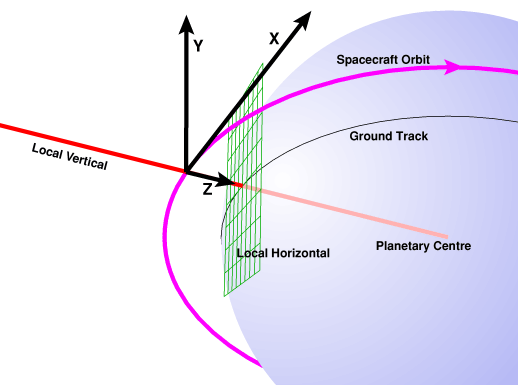
\includegraphics[width=0.5\textwidth]{figures/lvlh.png}
\caption{LVLH (Local vertical/local horizontal) is a frame of reference that is relative to a line drawn from the spacecraft to the centre of the body it is orbiting~\cite{lvlh}.}
\label{lvlh_diagram}
\end{center}
\end{figure}

Space is an extremely dangerous environment with many challenges of different natures and magnitudes. Some effects on a spacecraft can arise from radiation, space debris and micrometeorite impact, upper atmospheric drag, spacecraft electrostatic charging, and many other factors. While the resulting dynamics of these phenomena have various degrees of effect on a small spacecraft, these are outside the scope of this work. For the purposes of the study, all of these factors are ignored. It is assumed here that the spacecraft is operating under nominal conditions in an otherwise empty environment.

\subsection{Dynamical Equations of Motion} \label{cweqs}
The Clohessy-Wiltshire equations were used to model the dynamics of the spacecraft while it was in close proximity to the target vehicle. The Clohessy-Wiltshire equations describe a simplified model of orbital relative motion, in which the target is in a circular orbit, and the inspection spacecraft is in an elliptical or circular orbit. This model gives a first-order approximation of the chaser's motion in a target-centered coordinate system. It is used here in planning a rendezvous between the inspector and the target~\cite{cw_eqs}.

These equations of motion can be expressed as
\begin{equation}
\begin{split}
\ddot{x} &= 3n^2 + 2n\dot y \\
\ddot{y} &= -2n\dot x \\
\ddot{z} &= -n^2z
\end{split}
\end{equation}
and have the closed form solution given by
\begin{equation}
\begin{split}
x(t) = (4-3 \cos{(nt)})x_0 &+ \frac{\sin{(nt)}}{n}\dot x_0 + \frac{2}{n} (1 - \cos(nt))\dot y_0\\
y(t) = 6(\sin{(nt)}-nt)x_0 &+ y_0 \frac{-2}{n}(1 - \cos{(nt)})\dot x_0 \\
                         &+ \frac{4 \sin{(nt)} - 3nt}{n}\dot y_0 \\
z(t) = z_0 \cos{(nt)} &+ \frac{\dot z_0}{n} \sin{(nt)}
\end{split}
\end{equation}
where
\begin{equation}
n = \sqrt{\frac{\mu}{a^3_t}}
\end{equation}
and $a_t$ is the semi-major axis of the target vehicle's orbit, and $\mu$ is the standard gravitational parameter.

\section{Simulation}

\begin{figure}[tb]
\begin{center}
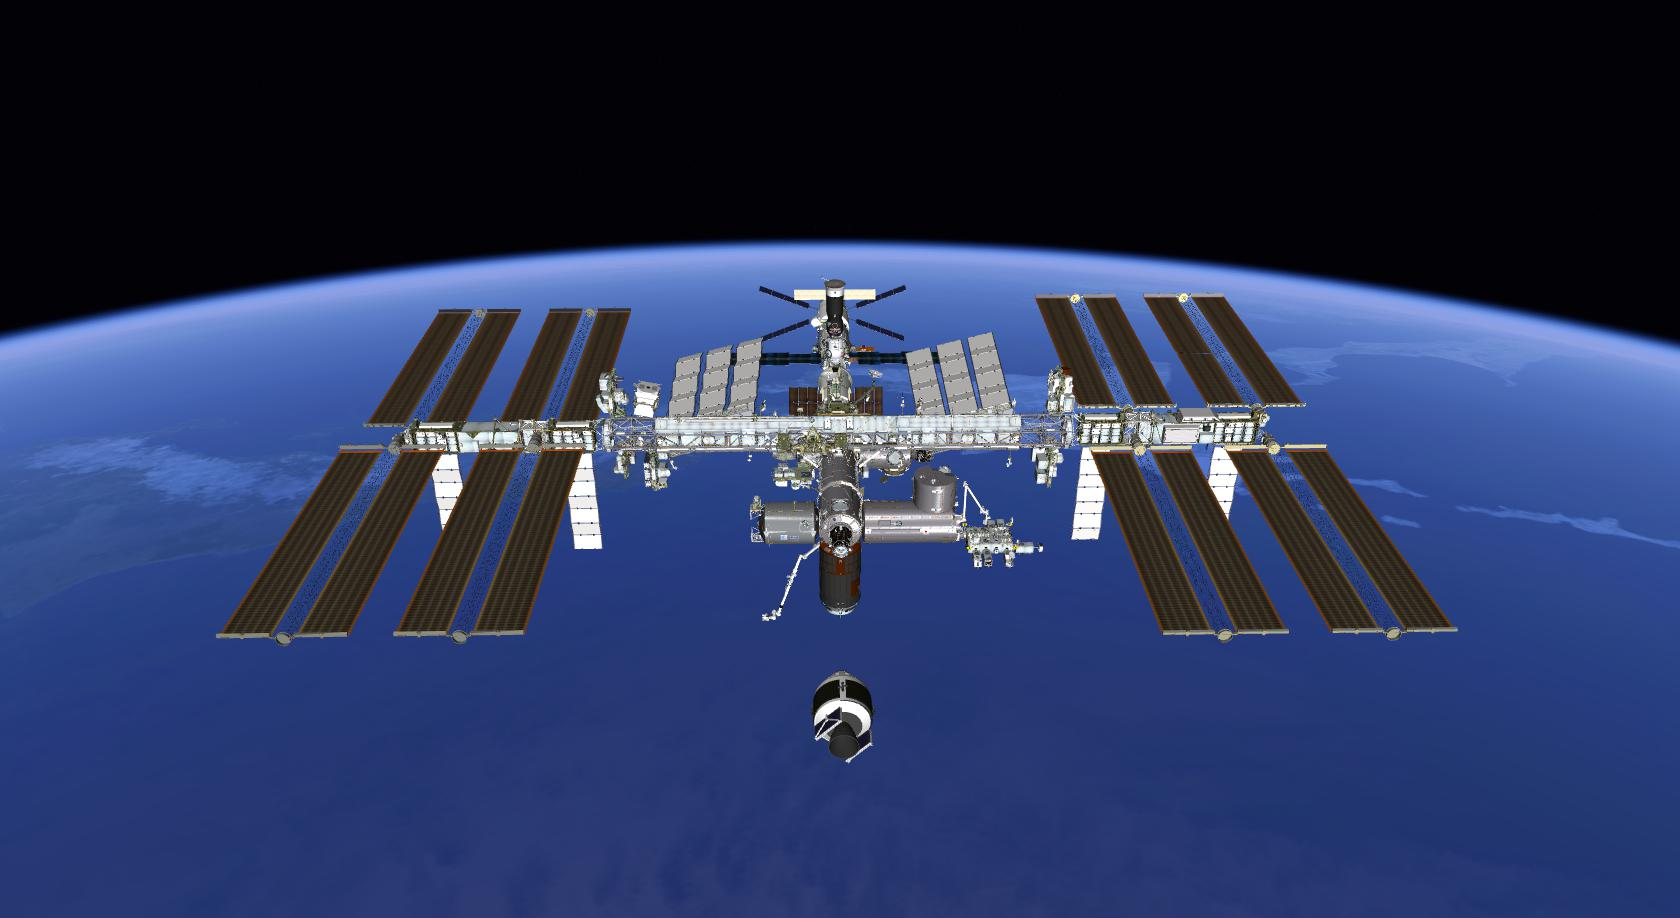
\includegraphics[width=0.5\textwidth]{figures/EDGE_ISS.jpeg}
\caption{Example EDGE visualization}
\label{edge_iss}
\end{center}
\end{figure}

The virtual simulation will be driven with a variety of software packages. The dynamics and control systems will be driven by several Python modules, while the visualization will be rendered in EDGE. EDGE is a graphics display tool developed at NASA's Johnson Space Center that combines key elements from graphics software developed for the space shuttle and the International Space Station programs, and adapts them for integration with other engineering simulations and facilities~\cite{EDGE}.

EDGE makes use of a node tree to structure data, objects, and models. Each node has many properties, the most notable of which are the node's position, orientation, and parent. Each node's position and orientation are defined relative to its parent's position and attitude. A node's parent can be changed to a different node, at which time the node's position and attitude are automatically updated to the correct values.

Three Python 2.7.9 scripts will be developed for use in the virtual simulation:
\begin{description}
    \item[\textbf{\textit{cv}}] \hfill \\
    A computer vision image processing module which takes advantage of OpenCV-Python version 2.4.9.
    \item[\textbf{\textit{dynamics}}] \hfill \\
    A dynamics and controls module.
    \item[\textbf{\textit{dcomm}}] \hfill \\
    A wrapper library developed to interface with EDGE's C++ DCOMM library.
\end{description}

\subsection{Python Modules}
\begin{figure}[b]
\begin{center}
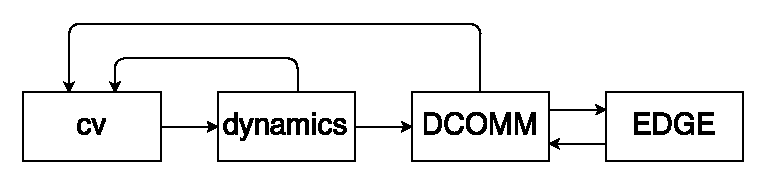
\includegraphics[width=0.5\textwidth]{figures/block.pdf}
\caption{Block diagram of software package interactions}
\label{block_diagram}
\end{center}
\end{figure}

\subsubsection{cv}
The \textit{cv} module takes advantage of Python bindings for OpenCV. OpenCV (Open Source Computer Vision) is a library of programming functions mainly aimed at real-time computer vision~\cite{opencv}. This module takes the live video feed from EDGE and attempts to identify features visible on the target spacecraft. The features of the target are supplied to the module a priori, and these descriptions were used to estimate the 3D pose of the target vehicle relative to the spacecraft's camera. This pose information is then passed on to the \textit{dynamics} module.

\subsubsection{dynamics}
The \textit{dynamics} module drives the dynamics and control of the simulation. The movement of the spacecraft around the target craft is modeled by the Clohessy-Wiltshire equations, see section~\ref{cweqs}. This module controls how the spacecraft operates in its different modes. This module will test several initial conditions and errors on the spacecraft while it operates under either of its two architectures.

\subsubsection{DCOMM}
The \textit{DCOMM} module was previously developed to network between Python scripts and EDGE. The Python DCOMM interface allows a user to call various C++ functions from EDGE's DCOMM module and communicate with an EDGE server. Users can move and rotate nodes, and can also change a node's parents, units, and principal axis definitions. Commands to set the spacecraft's attitude and position were sent from the \textit{dynamics} module through DCOMM and passed on to EDGE. This module was also responsible for requesting and handing off the video feed from the EDGE server.

\subsection{Sensors}
A system's sensors play an integral role when performing autonomous docking operations with a noncooperative target. As a result, a sensor's ability to accurately determine the system's range to target is imperative for mission success. In this simulation, an autonomous satellite conducts a docking operation with no \textit{a priori} knowledge of the target, and uses sensors to calculate a real-time orbital trajectory. Additionally, this simulation utilizes two different sensors, computer vision and laser range finder, for each robotic architecture from start to target capture. These results will be compared and discussed in Section~\ref{discuss}, and the superior sensor will be identified for each set of initial conditions.

\subsubsection{Computer Vision} \label{cv}
\begin{figure}[tbh]
\begin{center}
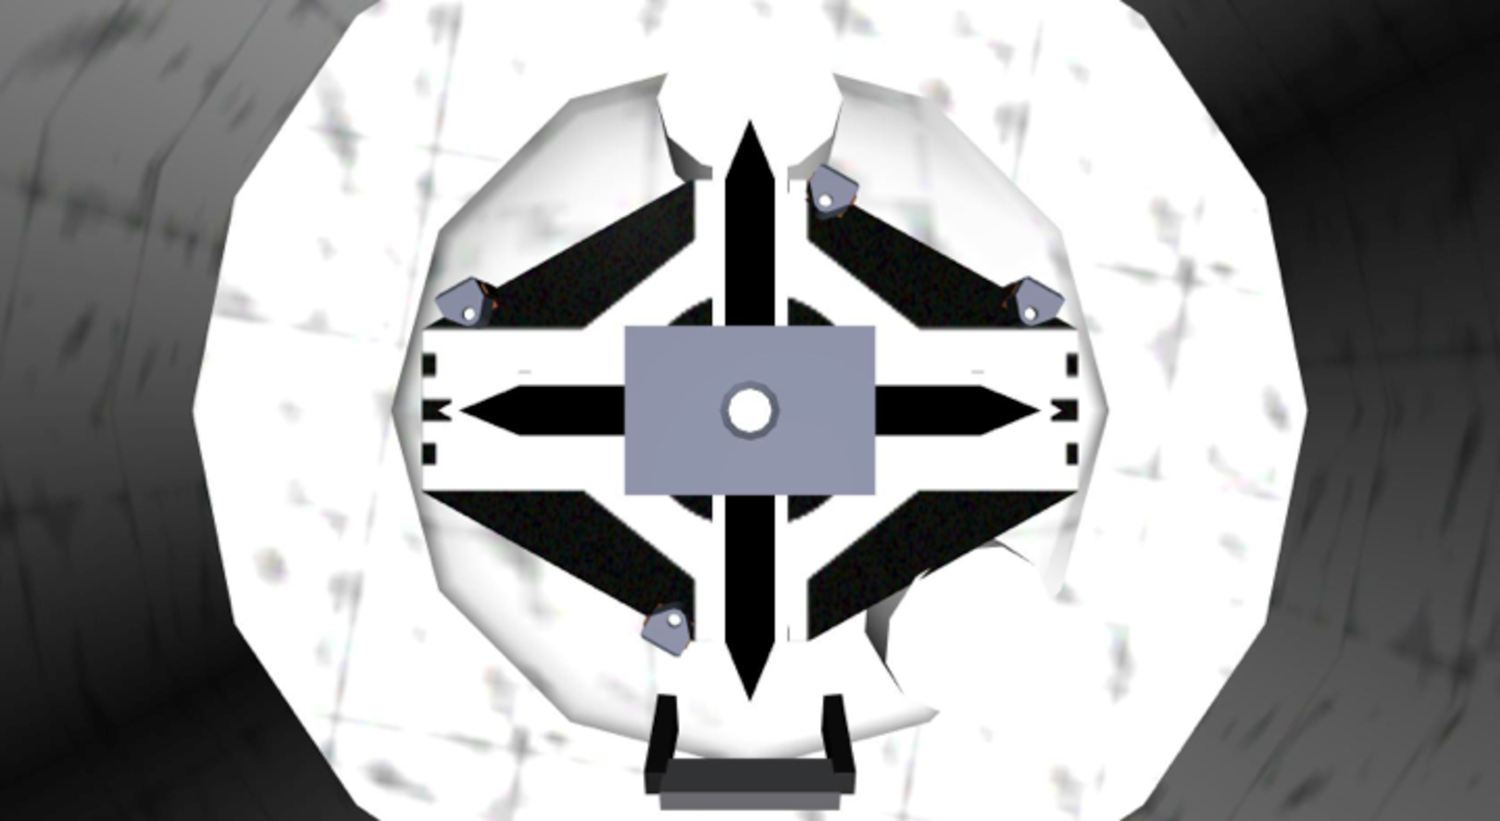
\includegraphics[width=0.5\textwidth]{figures/DockingPort.pdf}
\caption{Single picture taken from satellite}
\label{docking_port}
\end{center}
\end{figure}

\begin{figure}[tbh]
\begin{center}
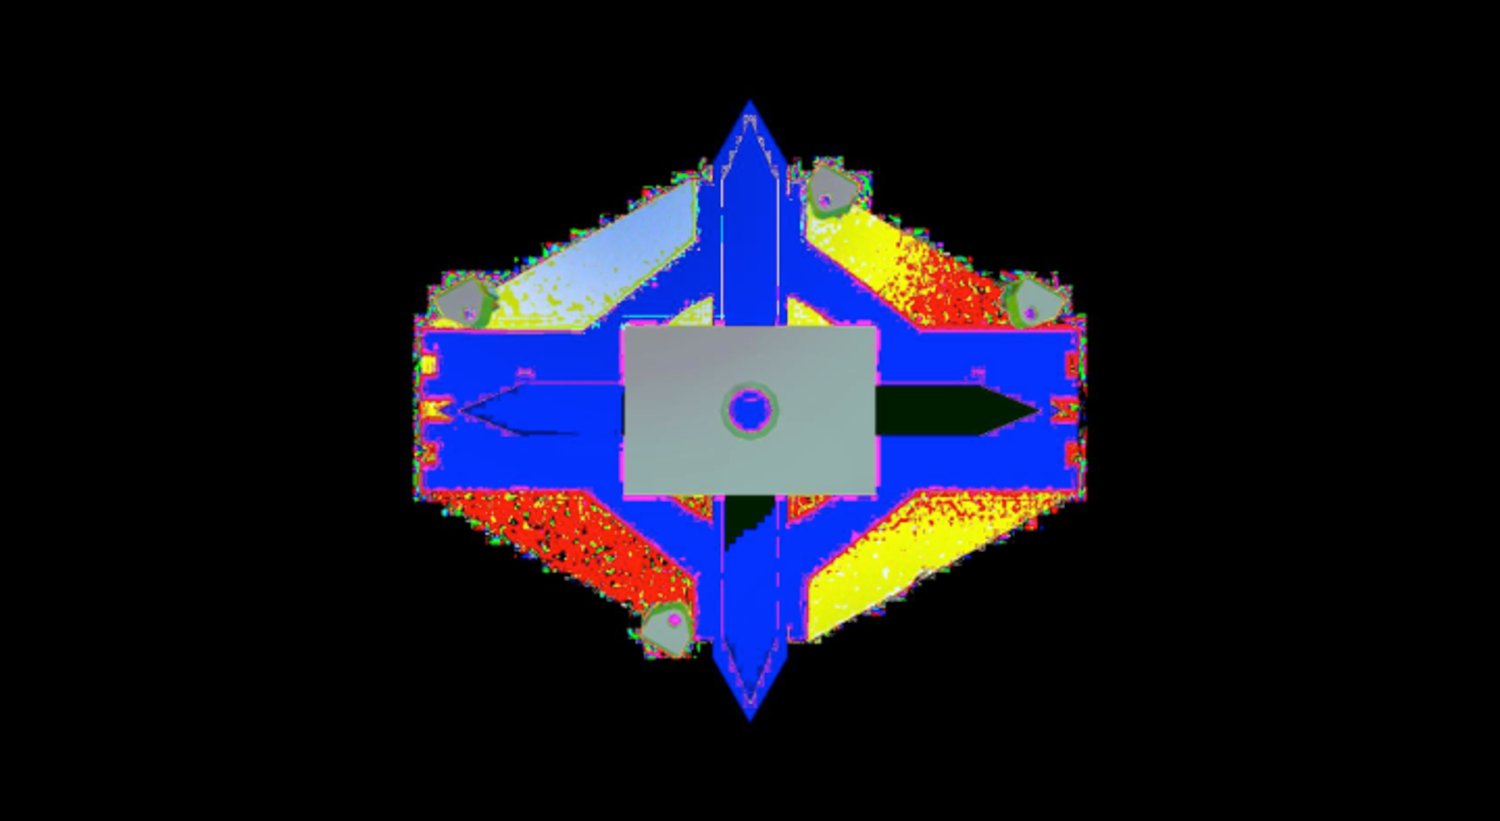
\includegraphics[width=0.5\textwidth]{figures/DockingPortSubtraction.pdf}
\caption{An identified docking port}
\label{docking_port_subtraction}
\end{center}
\end{figure}

\begin{figure}[tbh]
\begin{center}
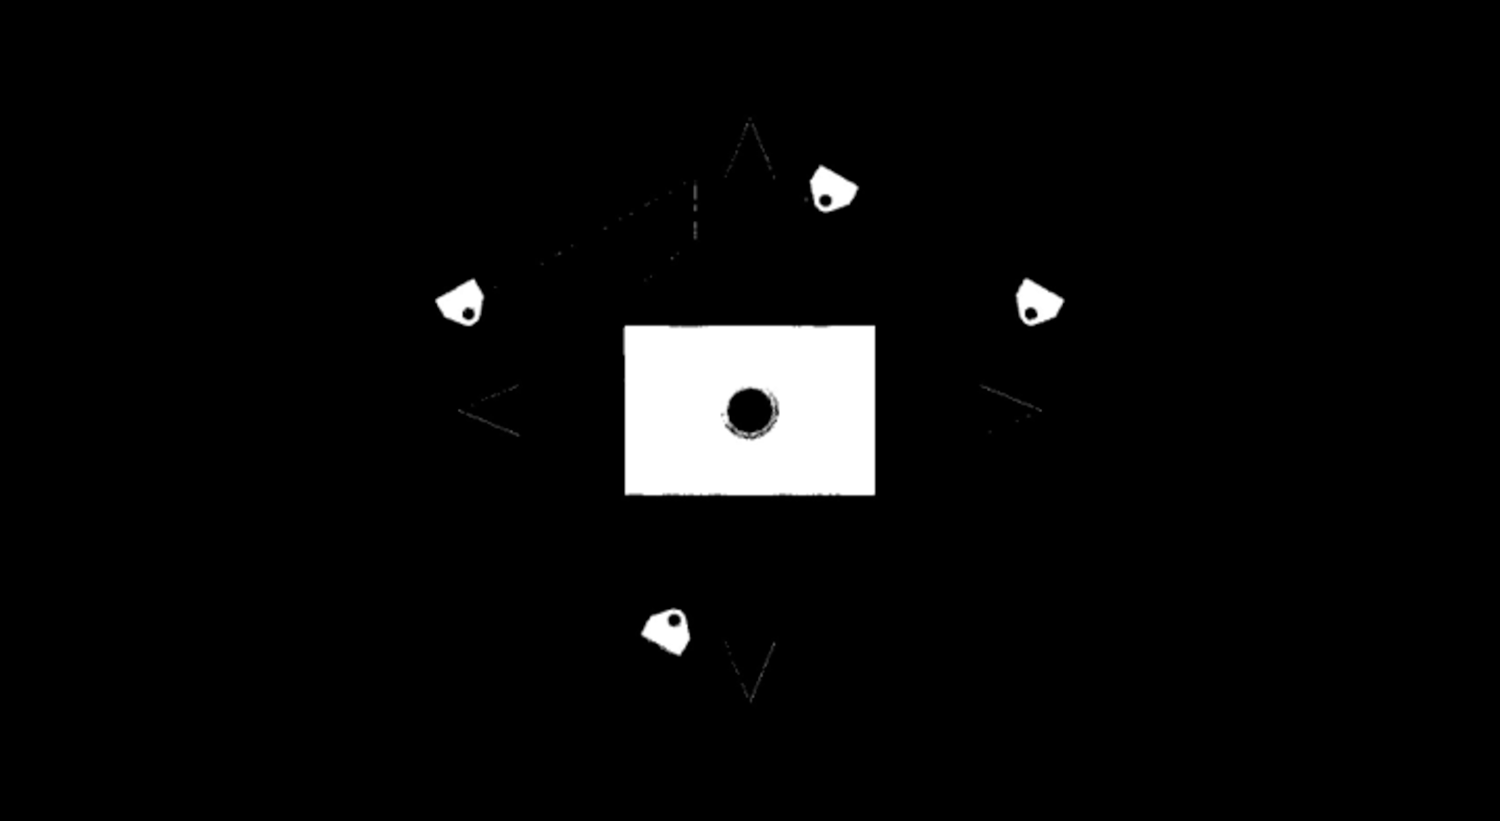
\includegraphics[width=0.5\textwidth]{figures/DockingPortFeatures.pdf}
\caption{Mask used to identify features on docking port}
\label{docking_port_features}
\end{center}
\end{figure}

The cameras on the spacecraft can serve the dual purpose of visual inspection and relative location estimation. The camera used in the simulation takes images of width 1600 pixels and height 900 pixels and performs several algorithms identify markers and estimate the relative location of the target spacecraft (an example image taken by the craft can be seen in Figure~\ref{docking_port}).

To identify the markers on the docking port, the spacecraft takes two pictures of the docking port, one with the satellites lights on, and the other with its lights off. The difference between these two images is used to identify the docking port (an example of the resultant image can be seen in Figure~\ref{docking_port_subtraction}). The highly reflective nature of the port makes it standout compared to the rest of the target. Certain predetermined color ranges are selected from the resultant image to create a mask identifying the 5 known markers (an example of the mask can be seen in Figure~\ref{docking_port_features}).

Contours are then extracted from the masked image using the algorithm described by Suzuki et al.~\cite{suzuki1985topological}. The size of these contours is then sorted from largest to smallest. The largest of these contours is assumed to be the largest of the markers. A clustering algorithm is then used to locate the next four largest markers that are roughly the same size. The area of these four markers is averaged, and this average is used to estimate the relative distance in the x direction. The offset of the center of the largest marker from the center of the image, combined with the estimated distance in the x direction, is used to estimate the relative distance in the y and z directions.

While this method proved effective a great majority of the time, it did occasionally lead to failures when the largest marker was misidentified. The error between the estimated state and the true state can be seen in Figure~\ref{error}. This error was comparable to the error for the laser sensor at large distances, but was quickly reduced to less than a few degrees for shorter distances.


\subsubsection{Laser Range Finder} \label{laser}
The second sensor that estimates the satellite's relative location is the laser range finder. Whenever a sensor tries to accurately estimate the position of its respective system, there is an innate measurement error, or ``noise,'' as a result of environmental disturbances and drift. To accurately simulate how noise effects the system, the simulation trials were first conducted using an exact laser range finder, and then again using a ``noisy'' laser sensor.

For the noisy laser range finder sensor, the current (x, y, z) position of the system is passed into the function, and noise is propagated throughout the system using a two-step method. First, error is added to the position by randomly generating a number between the positive and negative value of the predetermined laser error. Next, a secondary error is generated between the bounds of one plus/minus the laser error value. This secondary error is multiplied by the modified position, and these new x, y, and z values become the system's estimated position.  For this simulation, it is important to note that the predetermined laser error is manually set by the user, and thus varying the laser error will subsequently adjust the estimated position's magnitude.


\section{Robotic Architectures}
Two different robotic architectures were utilized in this simulation, deliberative and reactive, and both architectures were tested in unique trials using either the computer vision or the laser range finder sensors. Therefore for a given set of initial conditions, a minimum number of six trials were conducted: Deliberative -- Computer Vision, Deliberative -- Laser Range Finder (noisy), Deliberative -- Laser Range Finder (exact), Reactive -- Computer Vision, Reactive -- Laser Range Finder (noisy), and Reactive -- Laser Range Finder (exact). As previously mentioned, the results comparing both architectures, as well as both sensors, will be discussed in detail in Section ~\ref{discuss}.

\subsection{Deliberative Architecture}
\subsubsection{Overview}
A deliberative robotic architecture utilizes a hierarchical paradigm such that data is gathered to create a world model, and, after each iteration, this world model is updated before planning and calculating an action to take place. This architecture conducts steps in series, as opposed to parallel, and places a large emphasis on planning \cite{joshi}.

To mimic this paradigm, the deliberate architecture algorithm will consist of three states. The architecture will first Sense, and use sensors to determine the current state and to build the world model. The information gathered in Sense is passed on to Plan, which uses this information to determine parameters for an orbital maneuver. The Plan state will then pick one of three different trajectory types: Homing, Closing, Final Approach. Once this trajectory is planned, the trajectory is passed on to the Act state. The Act state performs open-loop thruster inputs. Once the burn is complete, the state switches back to Sense and the cycle continues until the target is reached.

\subsubsection{Algorithm}
As previously mentioned, the deliberative robotic architecture utilizes the Sense-Plan-Act paradigm, and its algorithm was intuitively organized in a similar manner. Below is a pseudo-code description of the three main functions that are used to build the world model, compute the desired trajectory, and conduct a corresponding burn.

\begin{description}
\item[\textbf{Sense}] \hfill \\
From the main simulation, an argument is passed into the sense function specifying which sensor, ``cv'', ``laser-noise'', or ``laser-exact'', will be utilized for this trial run. Using this specified argument, the sense function links the deliberative architecture simulation to its respective sensor, and the sensor updates the satellite's estimated state vector accordingly. Refer to Sections \ref{cv} and \ref{laser} for the respective details pertaining to the computer vision and laser range finder sensors.

\item[\textbf{Plan}] \hfill \\
Using the Sense estimated position values, Plan calculates the distance to target. If the distance is less than 127 cm, the satellite enters the Final Approach trajectory, with a burn time equal to 0.2s. Else if the distance to target is less than 1270 cm, the satellite enters the Closing trajectory and updates the burn time to equal 1.0s. Else, the satellite enters the Homing trajectory and utilizes a 5.0s burn time. Then after the appropriate trajectory and burn time have been selected, Plan computes the necessary burn needed to reach the target and perform the appropriate orbital maneuver.

\item[\textbf{Act}] \hfill \\
Act receives the calculated burn values from Plan, and decides if the specified thrust can be performed. If the desired burn rate is less than the minimum thrust, no burn is conducted. If the desired burn rate is within a specified value, allow the system to burn for a fraction of the desired burn rate. Else, if the desired burn rate is too large, conduct a burn equal to the previous burn rate. This particular series of checks prevents the satellite from performing large impractical burns, and it also makes the system's fuel burns more efficient. As Act is conducting this calculated burn, the satellite's position is simultaneously updated using the Clohessy-Wiltshire equations.
\end{description}

This algorithm will continue to perform in a Sense-Plan-Act cycle until the satellite has reached the target.

\subsection{Reactive Architecture}
\subsubsection{Overview}
Unlike the deliberative architecture, a reactive architecture eliminates planning, and thus operates without a global world model. Instead, this method utilizes a parallel approach, and uses a coupled Sense-Act relationship to quickly implement independent behaviors\cite{joshi}.

This reactive architecture algorithm makes use of a fuzzy approach where each behavior has a weighted contribution. In this paradigm, the robot takes sensing data and computes the best action to take independently of what the other behaviors decide to do. The robot will then do a combination of the possible behaviors. Four behaviors are currently planned: ``Move closer'', which uses no path planning, but attempts to get closer in LVLH frame; ``Don't hit'', which fires away from the target based off distance and relative velocity of the target; ``Station keeping'', which holds its position when the target region is reached, and ``Stay on orbit'', which pushes closer to the horizontal axis if the system is too far off the orbital path. The resulting thrust, $T$, is calculated by
\begin{equation}
T = \frac{ \sum^{n}_{i=0} T_i w_i} { \sum^{n}_{i=0} w_i },
\end{equation}
where $T_i$ is the thrust calculated by behavior $i$, $w_i$ is the weight of the behavior, and $n$ is the total number of behaviors.

\subsubsection{Algorithm}


\section{Simulation Results and Discussion} \label{discuss}
A complete simulation was conducted using an initial condition state vector such that the initial x displacement was equal to 254, 762, or 1270 cm; the initial y and z displacements were equal to 0, +/- 127, or +/- 93.98 cm; and the initial velocities were all equal to zero. All initial condition test combinations were simulated, creating a total of 27 different initial condition state vectors. The deliberative and reactive architecture algorithms were independently simulated for both the laser range finder and the computer vision sensors, and 10 trials were simulated for each initial condition state vector. A total of 1620 trial runs were conducted to test which sensor and architecture method achieved an optimal efficiency in fuel usage, time to completion, or both. Refer to Tables \ref{mean} and \ref{std_dev} for the mean value and standard deviations for the satellite's time to completion, the total delta v used, the radial distance from the docking port, and the ``rate,'' or total velocity, of the satellite when it reached the docking port. Additionally, refer to Table \ref{initial} for the mean and standard deviation for fuel usage given an initial state vector with zero y and z offsets.


% Mean table
\begin{table*}
\centering
\normalsize
\caption{Simulation Mean Value Results For All Trial Runs}
\begin{tabular}{llllll}
\toprule
Architecture & Sensor & Time (s) & Fuel (cm/s) & Distance (cm) & Rate (cm/s) \\
\midrule
Deliberative & cv & 353.307037  & 6.318384 & 0.001898 & 0.350590\\
			& laser (exact) & 353.503704 & 10.124424 & 0.001811 & 0.356138\\
			& laser (noisy) & 353.557407   & 9.219628 & 0.001824 & 0.351206\\
Reactive & cv & 371.858889  & 161.473580 & 0.303015 & 0.132178\\
& laser (exact) & 364.675926 & 49.945871 & 0.141140 & 0.127627\\
& laser (noisy) &  363.357407 & 277.725357 & 0.032213 & 0.410119 \\

\bottomrule
\end{tabular}
\label{mean}
\end{table*}

% Standard Deviation Table
\begin{table*}
\centering
\normalsize
\caption{Simulation Standard Deviation Results For All Trial Runs}
\begin{tabular}{llllll}
\toprule
Architecture & Sensor & Time (s) & Fuel (cm/s) & Distance (cm) & Rate (cm/s)\\
\midrule
Deliberative & cv & 166.281398 &  1.455229 & 0.001860 & 0.429374\\
			& laser (exact) & 166.424436 & 4.650075 & 0.001864 & 0.412567\\
& laser (noisy) & 166.462108 &  3.635545 & 0.002010 & 0.415513\\
Reactive & cv & 167.096079 & 72.930148 & 0.125167 & 0.079502\\
& laser (exact) & 167.232888 & 38.174648 & 0.043787 & 0.011663 \\
& laser (noisy) & 167.138923 & 130.190847 & 0.016381 & 0.209043 \\
\bottomrule
\end{tabular}
\label{std_dev}
\end{table*}




\subsection{Deliberative Architecture: Computer Vision vs. Laser Range Finder}

The deliberative algorithm was simulated for a total of 810 trials, and the means and standard deviations of its results were organized into Tables \ref{mean} and \ref{std_dev}, respectively. As seen in these tables, the computer vision (cv) and both laser range finder sensors (exact and noisy) had an average run time of approximately 353 seconds, with a standard deviation of about 166 seconds. For both time statistics, the cv was faster by approximately 0.02 seconds -- a slight difference that could essentially be attributed to calculation errors, and is thus too small to accurately distinguish which sensor performed with better time efficiency using the deliberative method.

Next, to determine which sensor was able to successfully dock the satellite, the final distance between the satellite and the docking port was measured. This distance should essentially go to zero, and as seen in Table \ref{mean}, all sensors successfully attained a small docking distance of approximately 0.0018 cm at an estimated rate of 0.35 cm/s. However, while the distribution of these three satellite-to-port distances is roughly equal to $8.7e-5$cm, the exact and noisy lasers had a greater mean fuel usage by about 4 cm/s and 3 cm/s, respectively, in comparison to the cv sensor. Furthermore both lasers' total fuel usage had a standard deviation equal to about 4.65 cm/s and 3.63 cm/s, whereas the computer vision had a standard deviation equal to about 1.46 cm/s, indicating the laser's fuel usage had a greater variance. These significant differences suggest that the computer vision sensor conducted more efficient delta v burns in comparison to the laser range finder sensor. Additionally, it is important to note that the noisy laser had a better fuel efficiency than the exact laser sensor -- an unexpected result seeing as the exact laser was simulated without added noise error, and thus mimics a ``perfect'' sensor.

 \begin{figure}
\begin{center}
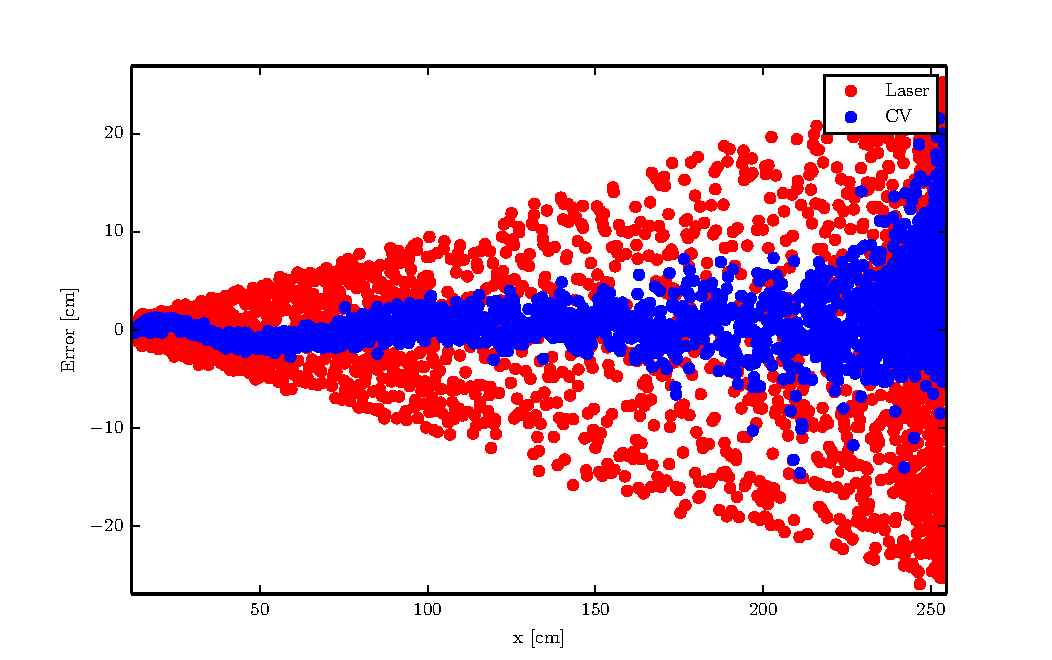
\includegraphics[width=0.5\textwidth]{figures/SensorErrors.pdf}
\caption{Sensor Errors}
\label{error}
\end{center}
\end{figure}

% fuel usage for initial offsets
\begin{table*}
\centering
\normalsize
\caption{Fuel Usage for a Subset of Simulation Trials}
\begin{tabular}{lllllll}
\toprule
Architecture & Sensor & x(cm) & y(cm) & z(cm) & Mean Fuel(cm/s) & Std. Dev Fuel (cm/s)\\
\midrule
Deliberative & cv & 254 &  0 & 0 & 5.873499 & 0.375036\\
& & 762 &  0 & 0 &  6.272073 & 0.434431\\
& & 1270 & 0 & 0 &  6.617597 &0.400670\\
			& laser (exact) & 254 & 0 & 0 &    5.810814 &0.399440\\
			& & 762 & 0 & 0 &    6.379098 &0.373520\\
			& & 1270 & 0 & 0 & 7.058843 & 0.484380\\
			& laser (noisy) & 254 & 0 & 0 &    5.780540 &0.383680\\
			& & 762 & 0 & 0 &    6.346101 &0.336987\\
			& & 1270 & 0 & 0 & 7.113471 &0.416979\\
\cmidrule(lr) {1-7}
Reactive & cv & 254 & 0 & 0 &   66.394292 &5.097201\\
& & 762 & 0 & 0 &   76.760390 & 4.843838\\
& & 1270 & 0 & 0 & 85.431635 &12.143697\\
& laser (exact) & 254 & 0 & 0 &   8.475532 & 0.060457\\
& & 762 & 0 & 0  &  15.361138 &0.104953\\
& & 1270 & 0 & 0 & 22.956919 & 0.235527\\
& laser (noisy) & 254 & 0 & 0 &  49.102620 & 2.463416\\
& & 762 & 0 & 0  &  58.001444 &2.857584\\
& & 1270 & 0 & 0 & 65.3067299 &2.863291\\
\bottomrule
\end{tabular}
\label{initial}
\end{table*}

To examine the mean fuel usage as a function of distance, Table \ref{initial} shows the mean fuel usage for both sensors when the only non-zero initial condition was the displacement along the x-direction. As the satellite is initially displaced farther from the target, the average total fuel consumption subsequently increases, and the difference between the cv's and the laser's fuel efficiency begins to increase as a function of distance. For example, when the satellite has a small initial displacement equal to 254 cm, the noisy laser sensor has the best performance with an average total burn rate of about 5.78 cm/s, followed by the exact laser sensor at 5.81 cm/s, and then finally the cv sensor with a burn rate of 5.87 cm/s. However, as the initial displacement between the satellite and the target increases to 762 cm, the ``most efficient'' sensor switches from the noisy laser range finder to the computer vision sensor, with an increased performance by about 0.074 cm/s. Then for the furthest offset of 1270 cm, this difference in fuel efficiency between the cv and noisy laser sensor increases by almost a factor of ten to 0.496 cm/s. Despite this distribution increase, the overall magnitude of this distribution was small, and essentially all three sensors had a comparable performance for this given set of initial conditions.

The main reason why the efficient sensor switches from the noisy laser range finder to the computer vision sensor is directly related to noise. When utilizing a computer vision sensor, an innate amount of natural error exists from computing image gradients and conducting Canny edge detection algorithms. Since computer vision has a substantial amount of preexisting noise, no additional noise was added to these measurements. However, since noise was only systematically added to the laser's position estimations, there exists a noticeable difference between the amount of error in the noisy laser's calculations as compared to those attained through computer vision. As seen in Figure \ref{error}, the laser's error has a canonical shape, where the cone has a larger error distribution the farther the satellite is displaced from the docking port. In comparison, the computer vision has a more refined error boundary region, exhibiting a slight sinusoidal behavior as the satellite is displaced closer to the target. Since the laser sensor has a larger error boundary, it is logical to conclude that this larger error was propagated, and created a higher fuel consumption from conducting a greater number of correction burns. To determine whether a reduction in added laser error would lead to a more optimal performance, an exact laser sensor was simulated. As discussed above, this exact laser surprisingly had the least efficient mean fuel usage for all time trials, and only performed the second best for a subset of trials in Table \ref{initial}. This suggests that the exact laser sensor's numerical computation errors, such as floating point round-off or truncation, were still above the cv's error threshold, and essentially allowed the computer vision to perform the best.


\begin{figure}[tb]
\begin{center}
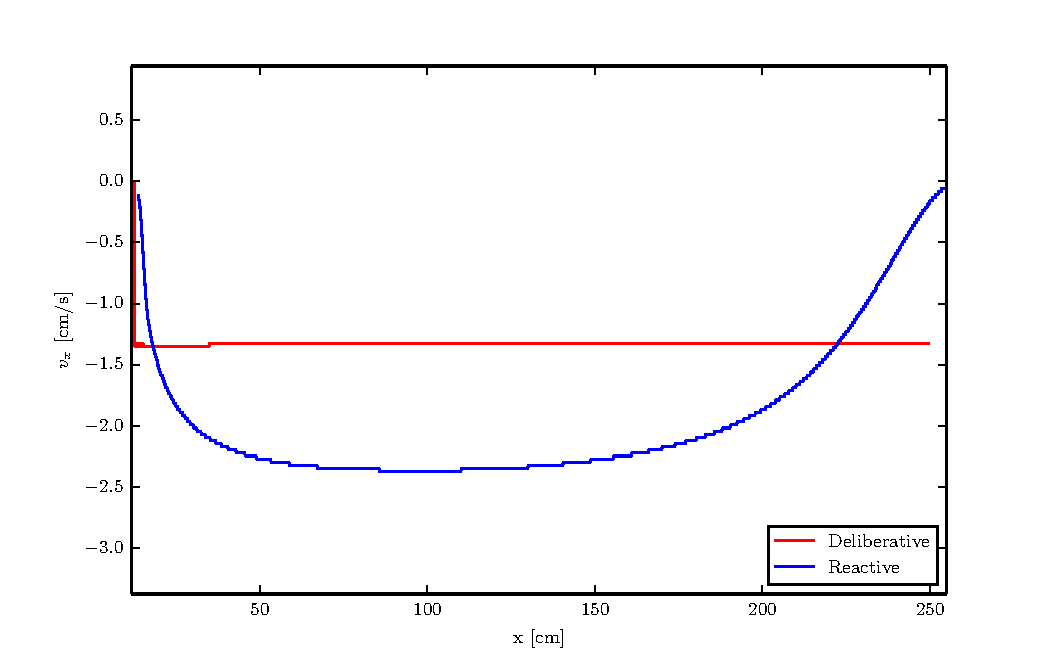
\includegraphics[width=0.5\textwidth]{figures/xVelocityClean.pdf}
\caption{X-Velocity for a Deliberative and Reactive Time Exact Laser Sensor Trial (100, 50, 37)}
\label{xClean_velocity}
\end{center}
\end{figure}

\begin{figure}[tb]
\begin{center}
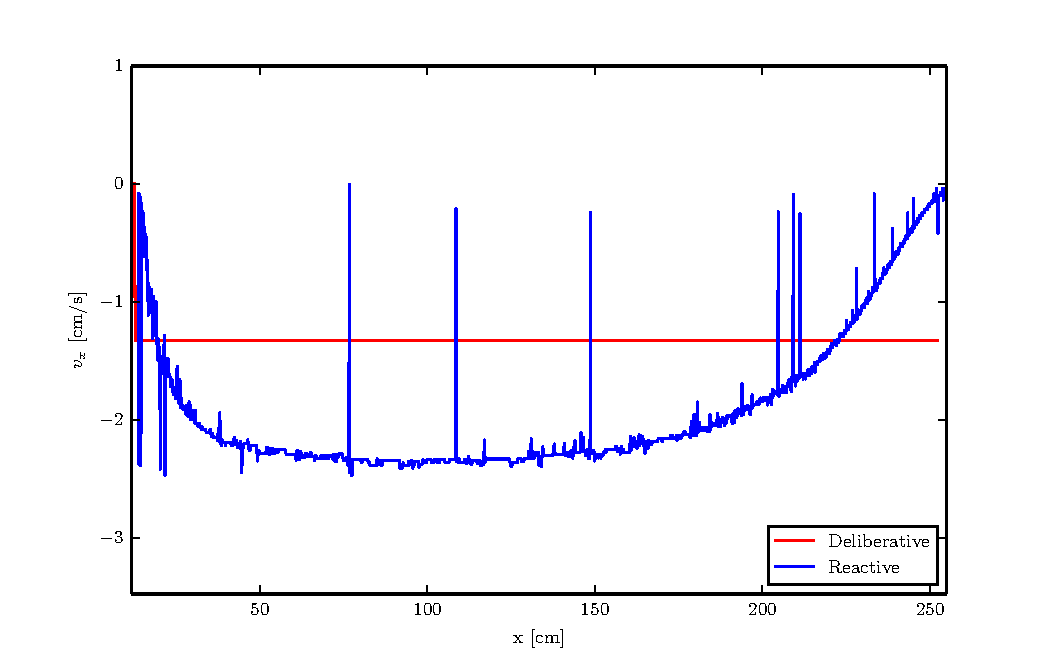
\includegraphics[width=0.5\textwidth]{figures/xVelocityNoisy.pdf}
\caption{X-Velocity for a Deliberative and Reactive Time Noisy Laser Sensor Trial (100, 50, 37)}
\label{xNoise_velocity}
\end{center}
\end{figure}

\begin{figure}[tb]
\begin{center}
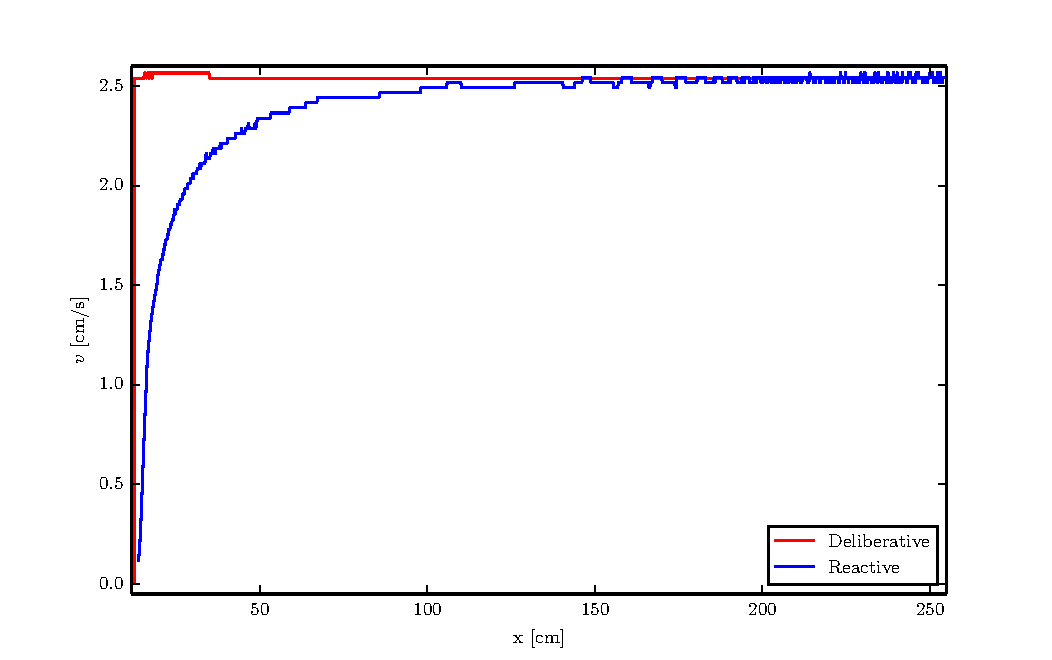
\includegraphics[width=0.5\textwidth]{figures/TotalVelocityClean.pdf}
\caption{Total Velocity Profile for a Deliberative and a Reactive Exact Laser Time Trial (100, 50, 37)}
\label{clean_total}
\end{center}
\end{figure}

\begin{figure}[tb]
\begin{center}
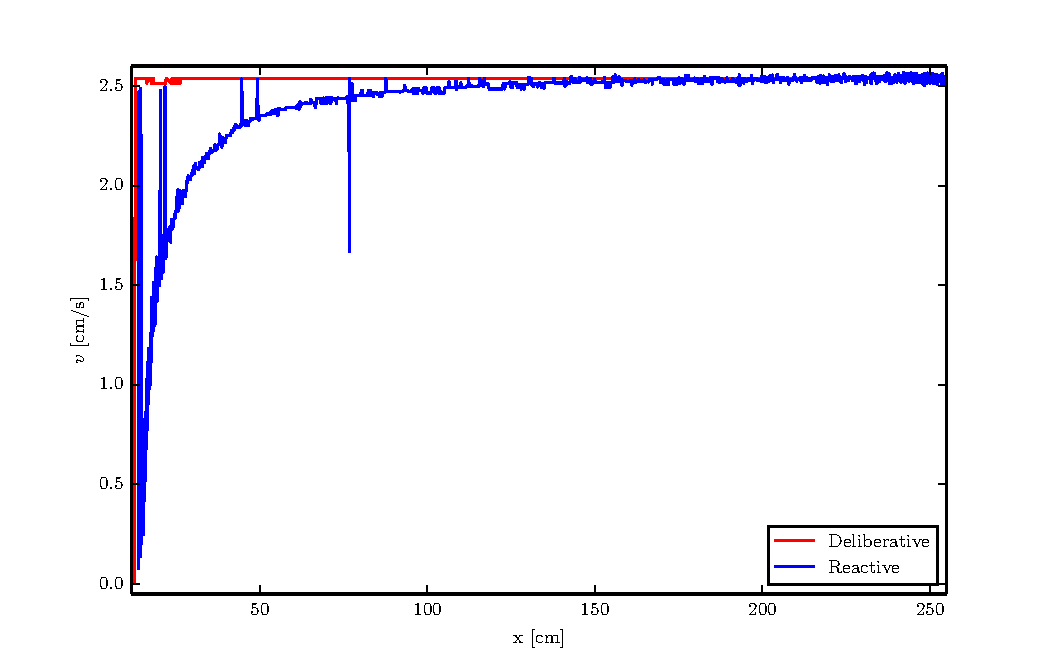
\includegraphics[width=0.5\textwidth]{figures/TotalVelocityNoisy.pdf}
\caption{Total Velocity Profile for a Deliberative and a Reactive Exact Laser Time Trial (100, 50, 37)}
\label{noisy_total}
\end{center}
\end{figure}
\subsection{Reactive Architecture: Computer Vision vs. Laser Range Finder}

\subsection{Deliberative vs. Reactive Architecture}

As seen in Tables \ref{mean} through \ref{initial}, the deliberative algorithm exhibits greater efficiency than the reactive algorithm for both the laser range finder and the computer vision sensors. For the average time to completion, the reactive algorithm exceeds the deliberative method's time by about 10 and 18 seconds for the laser (noisy and exact) and cv sensors, respectively. However, its standard deviation differs from the deliberative method's standard deviation by less than one second, indicating that significant outliers were not responsible for increasing the average time to completion. As a result of this longer flight time, the reactive method exhibits a significant loss in fuel efficiency. This inefficiency can be seen in Table \ref{mean} where the exact laser is the best performing sensor under the reactive method, utilizing an average total fuel of approximately 49.946 cm/s -- almost 5 times larger than the deliberative's comparable average fuel use of 10.124 cm/s. Furthermore, despite the reactive method's higher average fuel usage, the reactive method guides the satellite to an average final displacement that varies between 0.303 cm and 0.032 cm away from the target using the cv and laser sensors, respectively. These final displacements have a significant amount of error when compared to the small average displacements of 0.0018 cm for both deliberative sensors, reinforcing the final conclusion that the deliberative method exhibited greater time and fuel efficiency.

To compare the two architecture methods for a single trial run, refer to figures \ref{xClean_velocity}, \ref{xNoise_velocity}, \ref{clean_total} and \ref{noisy_total} where the system has an initial displacement of 254 cm, 127 cm, and 93.98 cm in the x, y, and z directions, respectively. As seen in Figures \ref{xClean_velocity} and \ref{xNoise_velocity}, the deliberative x-velocity profile maintains a relatively constant velocity of 1.27 cm/s as the satellite moves towards the docking port. When the satellite is approximately 2.54 cm from the target, the delta v burn goes to zero, and the satellite drifts into its final 0.0018 cm displacement. In comparison, the reactive x-velocity profile exhibits a dynamic response, with large velocity spikes under the noisy laser for the first 50 cm traveled along the x-direction. As the system continues to move closer, large velocity spikes occur intermittently for approximately every 50 cm between the 203 cm and 100 cm displacement points. Once the satellite reaches approximately 75 cm from the docking port, large delta v burns along the x-direction increase in frequency, with a final velocity spike at approximately 2.54 cm from target. As expected, the exact laser's x-velocity profile is a smoothed version of the noisy laser, omitting the large spikes in velocity since there was no added noise to the system.

If the total velocity profiles for each architecture is closely examined, the constant deliberative and the dynamic reactive velocity characteristics are reflected in figures \ref{clean_total} and \ref{noisy_total}. While the deliberative architecture appears to maintain its constant velocity profile and respective drop off at 2.54 cm, the reactive architecture's total velocity resembles a smooth and noisy exponential decay curve as the satellite moves in from its initial displacement under the exact and noisy lasers, respectively. As previously seen in the reactive's x-velocity profile, the system exhibits periodic large velocity spikes under the noisy laser, with a final velocity surge when the system is approximately 2.54 cm from target.

These results essentially reinforce the aforementioned claim that the reactive method does not take fuel efficiency into consideration when it computes its delta v burns. In order to compensate for the reactive method's position error, large correction burns are performed to redirect the satellite, and ultimately sacrifices the system's fuel efficiency in order to prevent a target collision. Therefore, while the reactive method is slightly faster to implement computationally, the deliberative method proves to have an increase in both overall performance and efficiency, and is thus the optimal choice for this simulation.




\section{Summary}

Through a virtual simulation environment, the authors will work to implement deliberative and reactive architectures to test an autonomous rendezvous docking algorithm. After reading previously conducted studies, the authors will strive to emulate a simplified SPHERES VERTIGO image-processing algorithm, and will test the algorithm using OpenCV and EDGE. Several trials will be conducted to compare these two architectures, and the system's initial conditions and errors will be varied in order to determine its overall effect on fuel usage and time to capture.


\section{Future Work}
Talk about applying a Kalman Filter to smooth out the results. Also mention how a KF would definitely improve the Reactive method, and would probably substantially decrease the total fuel usage under this method.

\nocite{*}
\bibliographystyle{IEEETran}
\bibliography{MAE252_Final_Paper}{}

\end{document}
